\section{Hops per Traceroute Measurement}

We want to look at traceroute measurements. The first thing we analyze is the
average number of hops per traceroute measurement. For that, we use the RIPE
Atlas built-in traceroute measurements. Figure~\ref{fig:hops-per-measument}
shows the histogram of hops for Canada, the United~Kingdom, France, and
Germany. The countries were chosen due to the completeness of the data. Similar
results were found when looking at other countries.

\begin{figure}
	\centering
	\begin{subfigure}[b]{\linewidth}
		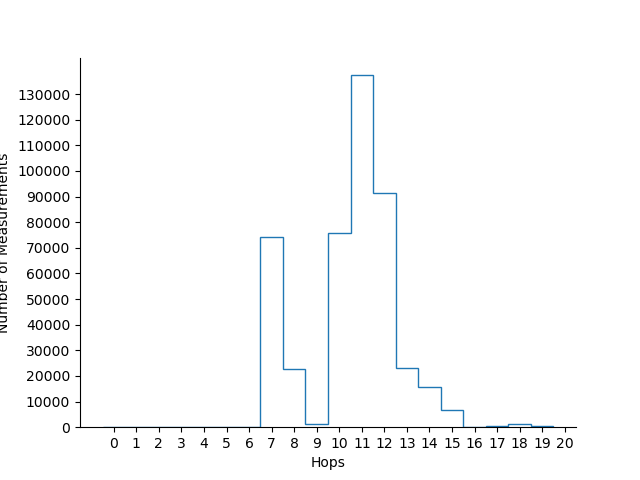
\includegraphics[width=\linewidth]{chapters/4-results/traceroute/img/hops_CA.png}
		\caption{Canada}
	\end{subfigure}
	\begin{subfigure}[b]{\linewidth}
		\includegraphics[width=\linewidth]{chapters/4-results/traceroute/img/hops_UK.png}
		\caption{United Kingdom}
	\end{subfigure}
	\begin{subfigure}[b]{\linewidth}
		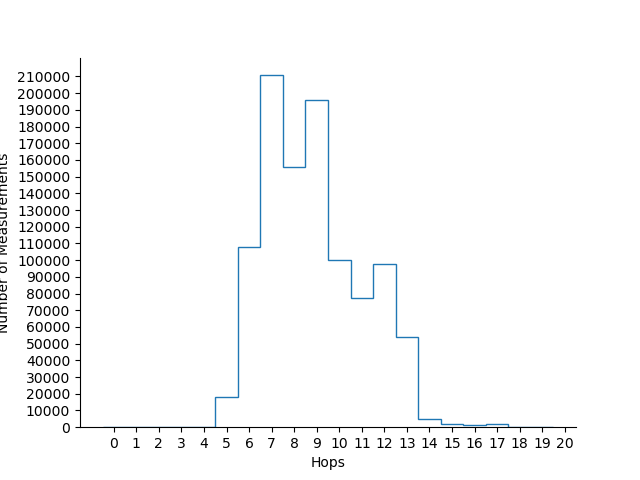
\includegraphics[width=\linewidth]{chapters/4-results/traceroute/img/hops_FR.png}
		\caption{France}
	\end{subfigure}
	\begin{subfigure}[b]{\linewidth}
		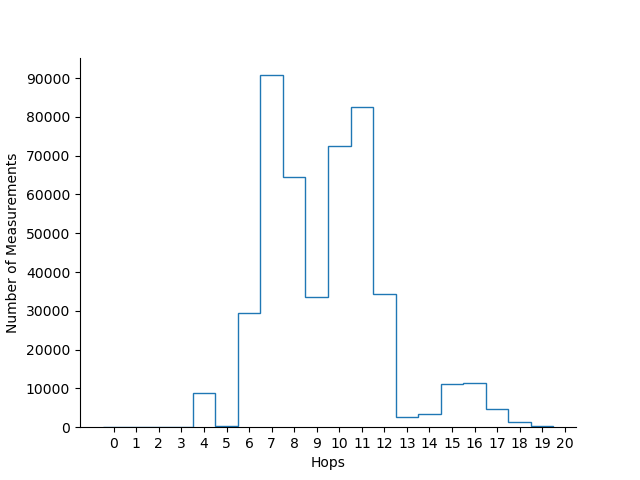
\includegraphics[width=\linewidth]{chapters/4-results/traceroute/img/hops_DE.png}
		\caption{Germany}
	\end{subfigure}
	\caption{Histogram of Hops the Traceroute Measurement took.}
	\label{fig:hops-per-measument}
\end{figure}

The histograms show that most routes take between seven and fourteen hops.
It is interesting to note that the histograms show a similar pattern compared
to the histogram for TLS handshake latencies that are shown in
Chapter~\ref{sec:latency-wholerange}. Both histograms have a pattern that
spikes at two points. We assume that there a specific reason for this
correlation that is part of the Starlink network.




